% Provenance (never printed): see sources/outline_sources.md (Year 3:
% atmospheric dynamics: vorticity and potential vorticity, Rossby waves,
% baroclinic instability, the general circulation and the Hadley cell).
% Brief: sources/book5/BRIEFS.md, ch. 20. Curves from
% figdata/bachelor-3/rossby_waves.py, eady.py and held_hou.py. Exercise and
% problem values in the Book 5 scratch calculator calc/ch20.py. The waves,
% shears and parcels of the exercises and the problem are invented.
\chapter{वायुमंडलीय गतिकी}\label{ch:b3:atmospheric-dynamics}

शीतकालीन मानचित्र पर ऊपरी क्षोभमंडल की जेट धारा ध्रुव के चारों ओर
कोई चिकनी वलय बनाकर नहीं घूमती। यह गोलार्ध के चारों ओर कुछ बड़ी तरंगों में टेढ़ी-मेढ़ी चलती है,
द्रोणियाँ उपोष्णकटिबंध की ओर पहुँचती हैं और कटक ध्रुव की ओर,
और पृष्ठ पर इनके नीचे अवदाब जन्म लेते हैं, कुछ दिनों तक बढ़ते हैं
और फिर समाप्त हो जाते हैं। ये तरंगें धीरे-धीरे खिसकती हैं,
कभी-कभी उस पवन के विपरीत भी, जो उन्हें लिए चलती है। इनकी संख्या,
इनकी चाल और इनके नीचे बनने वाले तूफ़ानों की वृद्धि
एक संरक्षित राशि से निकलती है, अंतरिक्ष से देखी गई वायु की भ्रमिलता से,
और उस ऊर्जा से जो अयन वृत्त और ध्रुवों के बीच तापमान के अंतर में संचित रहती है।

\begin{recall}
भ्रमिलता और परिसंचरण भौतिकी की पुस्तकों में हैं। ऊपरी क्षोभमंडल की रॉस्बी तरंगें, द्रोणियाँ और कटक,
बहिरुष्णकटिबंधीय चक्रवात और संख्यात्मक मौसम पूर्वानुमान का सिद्धांत
पुस्तक 4 (स्नातक वर्ष 2) में, मौसम तंत्रों वाले अध्याय में वर्णित हैं।
हैडली कोष्ठिका, फ़ेरेल और ध्रुवीय कोष्ठ, जेट धाराएँ,
पछुआ पवनें और वायु के एक वलय की कोणीय संवेग-जनित पवन पुस्तक 3 (स्नातक वर्ष 1) में,
वायुमंडल के सामान्य परिसंचरण वाले अध्याय में हैं,
और ऊष्मा का ध्रुवाभिमुख परिवहन उसके विकिरण और ऊष्मा परिवहन वाले अध्याय में है।
कोरिऑलिस प्राचल $f$, $\beta$-समतल,
रॉस्बी त्रिज्या और \omterm{thm:b3:gfd-foundations:thermal-wind}{ऊष्मीय पवन}
अध्याय~\ref{ch:b3:gfd-foundations} में हैं।
\end{recall}

\section{भ्रमिलता}\label{sec:b3:atmospheric-dynamics:vorticity}

किसी द्रव की भ्रमिलता, यानी उसके वेग का कर्ल, उसके स्थानीय
कोणीय वेग की दोगुनी होती है। बड़े पैमाने के वायुमंडल के लिए केवल उसका ऊर्ध्वाधर घटक मायने रखता है,
और उसमें पृथ्वी के घूर्णन का योगदान रहता है।

\begin{definition}[आपेक्षिक, ग्रहीय और निरपेक्ष भ्रमिलता]\label{def:b3:atmospheric-dynamics:vorticity-kinds}
क्षैतिज वेग $(u, v)$ के लिए \emph{आपेक्षिक
भ्रमिलता}\index{आपेक्षिक भ्रमिलता} भूमि के सापेक्ष वेग के कर्ल का ऊर्ध्वाधर घटक है,
$\zeta = \partial v/\partial x -
\partial u/\partial y$, जो ऊपर से देखने पर वामावर्त घूर्णन के लिए धनात्मक होती है।
\emph{ग्रहीय भ्रमिलता}\index{ग्रहीय भ्रमिलता} पृथ्वी के घूर्णन की भ्रमिलता का ऊर्ध्वाधर घटक है,
$2\Omega\sin\varphi =
f$। \emph{निरपेक्ष भ्रमिलता}\index{निरपेक्ष भ्रमिलता} इन दोनों का योग है,
$\zeta + f$।
\end{definition}

उत्तरी गोलार्ध में अवदाब, जहाँ वायु वामावर्त घूमती है,
$\zeta > 0$ रखता है और उसे चक्रवाती कहा जाता है; प्रतिचक्रवात का $\zeta < 0$ होता है।
\qty{15}{m/s} की पवन जब \qty{1000}{km} की वृत्ताकार परिधि पर घूमती है, तो ठोस घूर्णन में उसका $\zeta =
2V/R = \qty{3e-5}{s^{-1}}$ होता है, जो \ang{45} पर $f$ का एक तिहाई है:
अधिकतर ग्रहीय भाग ही बड़ा होता है।

\begin{theorem}[बैरोट्रॉपिक भ्रमिलता समीकरण]\label{thm:b3:atmospheric-dynamics:bve}
एक अश्यान, द्वि-आयामी प्रवाह में, जिसमें क्षैतिज अपसरण न हो और जो
$\beta$-समतल पर हो, प्रत्येक पार्सल की \omterm{def:b3:atmospheric-dynamics:vorticity-kinds}{निरपेक्ष भ्रमिलता} संरक्षित रहती है:
\[
\frac{\mathrm D(\zeta + f)}{\mathrm Dt} = 0 ,
\qquad\text{अर्थात}\qquad
\frac{\partial\zeta}{\partial t} + u\frac{\partial\zeta}{\partial x} + v\frac{\partial\zeta}{\partial y} + \beta v = 0 .
\]
यह \emph{बैरोट्रॉपिक भ्रमिलता समीकरण}\index{बैरोट्रॉपिक भ्रमिलता समीकरण} है।
\end{theorem}

\begin{proof}
क्षैतिज संवेग समीकरण हैं $\mathrm Du/\mathrm Dt - fv =
-(1/\rho_0)\partial p/\partial x$ और $\mathrm Dv/\mathrm Dt + fu =
-(1/\rho_0)\partial p/\partial y$। दूसरे को
$x$ के सापेक्ष और पहले को $y$ के सापेक्ष अवकलित करके घटाइए: दाब लुप्त हो जाता है।
$\delta = \partial u/\partial x + \partial v/\partial y$ लेने पर,
अभिवाही पद देते हैं $\partial_x(u\,\partial_xv + v\,\partial_yv) -
\partial_y(u\,\partial_xu + v\,\partial_yu) = u\,\partial_x\zeta +
v\,\partial_y\zeta + \zeta\delta$, और कोरिऑलिस पद $f\delta + \beta
v$ देते हैं। अतः $\mathrm D\zeta/\mathrm Dt + \beta v = -(\zeta + f)\,\delta$ प्राप्त होता है।
$\delta = 0$ के लिए, और चूँकि $\mathrm Df/\mathrm Dt = \beta v$, $\mathrm D(\zeta +
f)/\mathrm Dt = 0$ होता है।
\end{proof}

उपपत्ति से सामान्य नियम भी मिलता है, $\mathrm D(\zeta + f)/\mathrm Dt =
-(\zeta + f)\delta$: अभिसरण किसी स्तंभ को तेज़ घुमाता है, अपसरण उसे धीमा करता है,
जैसे कोई स्केटर बाँहें समेटने या फैलाने पर अपनी घूर्णन गति बदलता है। जिस परत की गहराई बदलती है,
वहाँ अभिसरण स्तंभ के खिंचाव से जुड़ा होता है, और
संरक्षित राशि एक अनुपात बन जाती है।

\begin{definition}[विभव भ्रमिलता]\label{def:b3:atmospheric-dynamics:pv}
\emph{विभव भ्रमिलता}\index{विभव भ्रमिलता} गहराई $h$ की समांगी परत के एक स्तंभ की
$q = (\zeta + f)/h$ होती है। सतत स्तरित द्रव में एर्टेल की विभव भ्रमिलता
$q = (\vec\omega_a\cdot
\nabla\theta)/\rho$ है, जहाँ $\vec\omega_a$ \omterm{def:b3:atmospheric-dynamics:vorticity-kinds}{निरपेक्ष भ्रमिलता} सदिश है और
$\theta$ विभव तापमान है।
\end{definition}

\begin{theorem}[विभव भ्रमिलता का संरक्षण]\label{thm:b3:atmospheric-dynamics:pv}
एक समांगी, द्रवस्थैतिक, अश्यान परत में, जिसकी परिवर्ती गहराई $h$ है और
जिसका क्षैतिज वेग ऊँचाई के साथ नहीं बदलता, $\mathrm Dq/\mathrm Dt = 0$
$q = (\zeta + f)/h$ के लिए होता है।
\end{theorem}

\begin{proof}
ऊपर की उपपत्ति से, $\mathrm D(\zeta + f)/\mathrm Dt = -(\zeta + f)\delta$।
एकसमान घनत्व के स्तंभ में द्रव्यमान संरक्षण से $\mathrm Dh/\mathrm
Dt = -h\delta$ मिलता है। तब $\mathrm Dq/\mathrm Dt = (1/h)\,\mathrm D(\zeta +
f)/\mathrm Dt - ((\zeta + f)/h^2)\,\mathrm Dh/\mathrm Dt = -(\zeta +
f)\delta/h + (\zeta + f)\delta/h = 0$।
\end{proof}

एर्टेल का रूप उसी तरह एक रुद्धोष्म, घर्षणरहित स्तरित द्रव प्रवाह में संरक्षित रहता है,
जिसमें स्थिर $\theta$ वाली दो सतहों के बीच की दूरी
$h$ की भूमिका निभाती है। वायु का एक स्तंभ, जो
पर्वत-श्रेणी पार करता है, चढ़ते समय दब जाता है: उसकी \omterm{def:b3:atmospheric-dynamics:vorticity-kinds}{निरपेक्ष भ्रमिलता} घटती है, वह
शिखर पर प्रतिचक्रवाती घूमता है, और फैलकर
पवन-पार्श्व में चक्रवाती रूप से घूमता है। निरपेक्ष
या \omterm{def:b3:atmospheric-dynamics:pv}{विभव भ्रमिलता} का संरक्षण अगले भाग की तरंगों का प्रत्यानयन तंत्र है,
जैसा नीचे का चित्र दिखाता है।

\begin{omfigure}
\begin{tikzpicture}[>=stealth, font=\small, declare function={w(\x)=0.9*sin(\x r);}]
\draw[black!40, dashed] (0,0) -- (12.6,0) node[right, font=\scriptsize] {अक्षांश $\varphi_0$};
\draw[thick, omDef, domain=0:12.566, samples=120] plot (\x, {w(\x)});
\foreach \x in {0.785, 2.356, 3.927, 5.498, 7.069, 8.639, 10.21, 11.78}
  \fill (\x, {w(\x)}) circle (0.06);
% crests: clockwise (anticyclonic), troughs: anticlockwise (cyclonic)
\foreach \x in {1.571, 7.854} {
  \draw[->, omThm, thick] (\x+0.45,{w(\x)+0.05}) arc (0:-300:0.45);
  \node[font=\scriptsize, omThm] at (\x,{w(\x)+0.75}) {$\zeta < 0$};}
\foreach \x in {4.712, 10.996} {
  \draw[->, omMeth, thick] (\x+0.45,{w(\x)-0.05}) arc (0:300:0.45);
  \node[font=\scriptsize, omMeth] at (\x,{w(\x)-0.75}) {$\zeta > 0$};}
\foreach \x in {3.1416, 9.4248} \draw[->, very thick] (\x,0.45) -- (\x,-0.45);
\foreach \x in {6.2832} \draw[->, very thick] (\x,-0.45) -- (\x,0.45);
\draw[->, thick] (8.4,-2.25) -- (6.4,-2.25) node[left, font=\scriptsize] {पैटर्न पश्चिम की ओर चलता है};
\draw[->] (0,-2.25) -- (1.4,-2.25) node[right, font=\scriptsize] {पूर्व};
\draw[->] (0,-2.25) -- (0,-1.65) node[above, font=\scriptsize] {उत्तर};
\end{tikzpicture}

\par\smallskip{\small रॉस्बी तरंग कैसे चलती है (योजनाबद्ध, उत्तरी
गोलार्ध)। अक्षांश $\varphi_0$ पर विराम में रखे कणों की एक श्रृंखला
एक तरंग में विस्थापित होती है। $\zeta + f$ के संरक्षण से, जो कण उत्तर की ओर हटते हैं, जहाँ
$f$ बड़ा है, उनमें घड़ी की सुई की दिशा में \omterm{def:b3:atmospheric-dynamics:vorticity-kinds}{आपेक्षिक भ्रमिलता} आती है; जो दक्षिण की ओर हटते हैं,
उनमें घड़ी की उलटी दिशा में। किसी शिखर और उसके पूर्व के गर्त के बीच प्रेरित प्रवाह
दक्षिण की ओर है, और गर्त तथा उसके पूर्व के शिखर के बीच उत्तर की ओर (काले
तीर); प्रत्येक शिखर के पश्चिम में विस्थापन बढ़ता है और पूरा पैटर्न
पश्चिम की ओर खिसकता है।}\label{fig:b3:atmospheric-dynamics:restoring}
\end{omfigure}

\section{रॉस्बी तरंगें}\label{sec:b3:atmospheric-dynamics:rossby}

पुस्तक 4 (स्नातक वर्ष 2) में ऊपरी क्षोभमंडल की रॉस्बी तरंगों का वर्णन किया गया था।
\omterm{thm:b3:atmospheric-dynamics:bve}{बैरोट्रॉपिक भ्रमिलता समीकरण} इनकी व्याख्या करता है। प्रवाह को एकसमान पश्चिमी
$U$ और धारा-फलन $\psi'$ वाले एक छोटे विक्षोभ के योग के रूप में लिखिए, ताकि
$u' = -\partial\psi'/\partial y$, $v' = \partial\psi'/\partial x$ और $\zeta'
= \nabla^2\psi'$ हों।

\begin{theorem}[रॉस्बी तरंगों का परिक्षेपण]\label{thm:b3:atmospheric-dynamics:rossby}
छोटे विक्षोभ $\psi' \propto \mathrm e^{\mathrm i(kx + ly - \omega t)}$, जो
$U$ वाली एकसमान पश्चिमी पवन में, $\beta$-समतल पर, हों, वे
\emph{रॉस्बी-तरंग परिक्षेपण संबंध}\index{रॉस्बी-तरंग परिक्षेपण संबंध} का पालन करते हैं:
\[
\omega = Uk - \frac{\beta k}{k^2 + l^2} .
\]
इनका पूर्व की ओर कला-वेग $c = \omega/k = U - \beta/K^2$ है, जहाँ $K^2 =
k^2 + l^2$ है, और इनका पूर्व की ओर समूह-वेग $c_g = \partial\omega/\partial
k = U + \beta(k^2 - l^2)/K^4$ होता है।
\end{theorem}

\begin{proof}
$U$ के सापेक्ष रैखिकृत करने पर \omterm{thm:b3:atmospheric-dynamics:bve}{बैरोट्रॉपिक भ्रमिलता समीकरण}
$(\partial_t + U\partial_x)\nabla^2\psi' + \beta\,\partial_x\psi' = 0$ हो जाता है, जहाँ
छोटी राशियों के गुणनफल हटा दिए गए हैं और मूल प्रवाह का $\zeta$
शून्य माना गया है। समतल तरंग के लिए $\partial_t \to -\mathrm i\omega$,
$\partial_x \to \mathrm ik$ और $\nabla^2 \to -K^2$ लेने पर $(-\mathrm i\omega +
\mathrm iUk)(-K^2) + \mathrm i\beta k = 0$ प्राप्त होता है, अर्थात् $(\omega - Uk)K^2 =
-\beta k$। $\omega$ का $k$ के सापेक्ष अवकलन करने पर $c_g = U -
\beta/K^2 + 2\beta k^2/K^4$ मिलता है, जो दिया गया रूप है।
\end{proof}

\begin{omfigure}
\begin{tikzpicture}
\begin{groupplot}[group style={group size=2 by 1, horizontal sep=1.7cm},
  width=0.48\linewidth, height=0.46\linewidth, tick label style={font=\scriptsize},
  label style={font=\small}, legend style={font=\scriptsize, draw=none, fill=none}]
\nextgroupplot[xlabel={आंचलिक तरंग-संख्या $n$}, ylabel={गति (\unit{m/s})},
  xmin=1, xmax=12, ymin=-40, ymax=60, legend pos=north east, legend cell align=left,
  title={\small \ang{45} N}]
% computed in figdata/bachelor-3/rossby_waves.py
\addplot[omThm, thick] table[x=n, y=c15] {figdata/out/bachelor-3-rossby_waves-disp.dat};
\addlegendentry{$c$, $U = 15$}
\addplot[omThm, thick, densely dashed] table[x=n, y=cg15] {figdata/out/bachelor-3-rossby_waves-disp.dat};
\addlegendentry{$c_g$, $U = 15$}
\addplot[omDef, thick] table[x=n, y=c0] {figdata/out/bachelor-3-rossby_waves-disp.dat};
\addlegendentry{$c$, $U = 0$}
\addplot[omDef, thick, densely dashed] table[x=n, y=cg0] {figdata/out/bachelor-3-rossby_waves-disp.dat};
\addlegendentry{$c_g$, $U = 0$}
\addplot[black!50, thin, domain=1:12, samples=2, forget plot] {0};
\nextgroupplot[xlabel={अक्षांश (\unit{\degree} N)}, ylabel={स्थिर तरंग-संख्या $n_s$},
  xmin=20, xmax=75, ymin=0, ymax=9, legend pos=north east, legend cell align=left]
\addplot[omMeth, thick] table[x=lat, y=n10] {figdata/out/bachelor-3-rossby_waves-stat.dat};
\addplot[omDef, thick] table[x=lat, y=n15] {figdata/out/bachelor-3-rossby_waves-stat.dat};
\addplot[omThm, thick] table[x=lat, y=n20] {figdata/out/bachelor-3-rossby_waves-stat.dat};
\addplot[black, only marks, mark=*, mark size=1.1pt] table[x=lat, y=ns] {figdata/out/bachelor-3-rossby_waves-statobs.dat};
\legend{\qty{10}{m/s}, \qty{15}{m/s}, \qty{20}{m/s}, जनवरी \qty{300}{hPa}}
\end{groupplot}
\end{tikzpicture}

\par\smallskip{\small बाएँ, पूर्व की ओर कला-वेग $c$ (ठोस) और समूह-वेग
$c_g$ (बिंदीदार) रॉस्बी तरंगों का, $l = 0$ के साथ, \ang{45} N पर,
अक्षांश-वृत्त के चारों ओर तरंगों की संख्या के विरुद्ध, बिना माध्य पवन के (नीला)
और \qty{15}{m/s} की पश्चिमी पवन में (लाल): लंबी तरंगें पश्चिम की ओर चलती हैं, छोटी
पूर्व की ओर ले जाई जाती हैं, और $c_g > c$। दाएँ, 10, 15 और \qty{20}{m/s} की एकसमान पश्चिमी पवनों के लिए स्थिर तरंग-संख्या,
और जनवरी की
आंचलिक-माध्य पवन \qty{300}{hPa} पर प्रत्येक अक्षांश के लिए (बिंदु, NCEP--NCAR
रीएनालिसिस~1, 1991--2020)।}\label{fig:b3:atmospheric-dynamics:rossby}
\end{omfigure}
% ledger: data:b5-ncep-uwnd, geod5:grs80-defining, earth:Rmean

वायु के सापेक्ष तरंगें सदा पश्चिम की ओर चलती हैं, और जो तरंग जितनी लंबी होती है
वह उतनी ही तेज़ चलती है। एक पश्चिमी पवन छोटी तरंगों को पूर्व की ओर ले जाती है; लंबी तरंगों को वह
नहीं ले जा पाती, और वे उसके विरुद्ध पश्चिम की ओर बहती हैं। इन दोनों के बीच
एक लंबाई स्थिर रहती है।

\begin{proposition}[स्थिर रॉस्बी तरंगें]\label{prop:b3:atmospheric-dynamics:stationary}
एक पश्चिमी पवन $U > 0$ में, जिस तरंग में कोई याम्योत्तर संरचना नहीं है ($l = 0$), वह
तब स्थिर होती है जब उसकी तरंगदैर्घ्य \emph{स्थिर रॉस्बी
तरंगदैर्घ्य}\index{स्थिर रॉस्बी तरंगदैर्घ्य} $\lambda_s =
2\pi\sqrt{U/\beta}$ हो। अक्षांश-वृत्त $\varphi$ के चारों ओर यह तरंगों की एक पूर्ण
संख्या है, जो $n_s = \sqrt{2\Omega a\cos^3\varphi/U}$ के निकट है।
\end{proposition}

\begin{proof}
$c = 0$ जब $k^2 = \beta/U$ हो, तब $\lambda_s = 2\pi/k = 2\pi\sqrt{U/\beta}$ होता है।
वृत्त की लंबाई $2\pi a\cos\varphi$ है, इसलिए $n_s = a\cos\varphi\,k =
a\cos\varphi\sqrt{2\Omega\cos\varphi/(aU)} = \sqrt{2\Omega a\cos^3\varphi/U}$।
\end{proof}

\ang{45} N पर \qty{15}{m/s} की पश्चिमी पवन में, जिसमें $\beta =
\qty{1.62e-11}{m^{-1}.s^{-1}}$, $\lambda_s = \qty{6050}{km}$ और $n_s =
4.7$: गोलार्ध के चारों ओर चार या पाँच तरंगें आती हैं। \omterm{def:b3:atmospheric-dynamics:eddy}{आंचलिक माध्य}
जनवरी पवन \qty{300}{hPa} पर, \ang{45} N पर लगभग \qty{21}{m/s}, जहाँ $n_s$
\ang{35} से \ang{55} N तक लगभग चार है, और ध्रुव की ओर घटता है।
$l = 0$ वाली तरंग का समूह वेग उसकी कला वेग से $2\beta/k^2$ अधिक होता है: ऊर्जा
तरंग से आगे दौड़ती है, इसलिए एक स्थान पर उठा विक्षोभ उसके प्रवाह की दिशा में नए गर्त
और कटक बनाता है, कुछ दिनों बाद और हज़ारों किलोमीटर पूर्व में, जबकि
स्वयं प्रतिरूप मुश्किल से खिसकता है। पर्वत-श्रेणियाँ और
महाद्वीपों और महासागरों के बीच तापमान के अंतर ठीक इसी प्रकार की स्थिर
तरंगों को, \omterm{def:b3:atmospheric-dynamics:pv}{विभव भ्रमिलता} के खिंचाव और संपीड़न के माध्यम से,
उत्पन्न करते हैं।
% ledger: geod5:grs80-defining, earth:Rmean, data:b5-ncep-uwnd (values in figdata/bachelor-3/rossby_waves.py)


\section{बैरोक्लिनिक अस्थिरता}\label{sec:b3:atmospheric-dynamics:baroclinic}

पिछले भाग की तरंगें उदासीन हैं: न वे बढ़ती हैं, न क्षीण होती हैं।
मध्य अक्षांशों के तूफ़ान बढ़ते हैं, और अपनी ऊर्जा
\omterm{thm:b3:gfd-foundations:thermal-wind}{ऊष्मीय पवन} जिस तापमान-अंतर को व्यक्त करती है, उससे खींचते हैं।

\begin{definition}[उपलब्ध स्थितिज ऊर्जा]\label{def:b3:atmospheric-dynamics:ape}
\emph{उपलब्ध स्थितिज ऊर्जा}\index{उपलब्ध स्थितिज ऊर्जा} किसी स्तरित द्रव की
उसकी कुल स्थितिज ऊर्जा (गुरुत्वीय और आंतरिक) और
उसके द्रव्यमान के रुद्धोष्म पुनर्विन्यास से वह जितनी न्यूनतम कुल स्थितिज ऊर्जा
तक पहुँच सकता है, उन दोनों का अंतर है: वह अवस्था जिसमें
नियत विभव तापमान, या विभव घनत्व, के पृष्ठ
क्षैतिज होते हैं।
\end{definition}

क्षैतिज समएन्ट्रॉपी-पृष्ठों वाले द्रव में \omterm{def:b3:atmospheric-dynamics:ape}{उपलब्ध स्थितिज ऊर्जा} नहीं होती, चाहे
उसमें कितनी भी स्थितिज ऊर्जा हो; वह द्रव जिसके समएन्ट्रॉपी-पृष्ठ झुके हों, एक ओर गर्म और हल्का, दूसरी ओर ठंडा
और सघन, उन्हें नीचे खिसकने देकर कुछ ऊर्जा मुक्त कर सकता है। दो वायु-पार्सलों का
आदान-प्रदान दिखाता है कि यह कैसे होता है। मान लीजिए भूमध्य की ओर निचले भाग में एक गर्म पार्सल और
ध्रुव की ओर ऊपरी भाग में एक ठंडा पार्सल, दोनों एक ही समएन्ट्रॉपी-पृष्ठ पर, एक स्थिर
वायुमंडल में, जिसके समएन्ट्रॉपी-पृष्ठ ध्रुव की ओर उठते हैं। उन्हें समएन्ट्रॉपी-पृष्ठ के साथ
बदलने से कुछ नहीं बदलता। समएन्ट्रॉपी-पृष्ठ से कम ढलान वाले पथ पर उन्हें बदलने से
गर्म पार्सल ऊपर और ध्रुव की ओर उस हवा में पहुँचता है जो स्वयं उससे ठंडी है,
और ठंडा पार्सल नीचे और भूमध्य की ओर अधिक गर्म हवा में पहुँचता है: गर्म ऊपर
उठता है, ठंडा नीचे धँसता है, द्रव्यमान-केंद्र नीचे गिरता है, और गतिज
ऊर्जा मुक्त होती है। क्षैतिज और समएन्ट्रॉपी-पृष्ठों के बीच इस पच्चर के भीतर के पथ
ऊर्जा मुक्त करते हैं; मध्य अक्षांशों के \omterm{def:b3:atmospheric-dynamics:eddy}{भँवर} ऐसे आदान-प्रदान हैं जो ऊष्मा
ध्रुव की ओर और ऊपर ले जाते हैं।

\begin{definition}[बैरोक्लिनिक अस्थिरता]\label{def:b3:atmospheric-dynamics:baroclinic-instability}
\emph{बैरोक्लिनिक अस्थिरता}\index{बैरोक्लिनिक अस्थिरता} ऊष्मीय पवन-संतुलन में
स्थित एक घूर्णनशील, स्तरित प्रवाह की अस्थिरता है, जिसके द्वारा
विक्षोभ, झुके समएन्ट्रॉपी-पृष्ठों की \omterm{def:b3:atmospheric-dynamics:ape}{उपलब्ध स्थितिज ऊर्जा} को
अपनी ही गतिज ऊर्जा में बदलकर बढ़ते हैं।
\end{definition}

\begin{definition}[ईडी मॉडल]\label{def:b3:atmospheric-dynamics:eady}
\emph{ईडी मॉडल}\index{ईडी मॉडल} $f$-समतल पर दो कठोर क्षैतिज पृष्ठों के बीच
$z = 0$ और $z = H$ पर स्थित एक बूसिनेस्क द्रव है, जिसमें एकसमान
\omterm{def:b3:gfd-foundations:buoyancy}{उत्प्लावन आवृत्ति} $N$ है और ऊँचाई के साथ रैखिक रूप से बढ़ती एक पश्चिमी पवन,
$U = \Lambda z$, जो ध्रुव की ओर एकसमान तापमान-ह्रास के साथ ऊष्मीय पवन-संतुलन में है;
इसके विक्षोभ अर्ध-भू-विक्षेपी
समीकरणों का पालन करते हैं।
\end{definition}

\begin{theorem}[ईडी वृद्धि दर]\label{thm:b3:atmospheric-dynamics:eady}
\omterm{def:b3:atmospheric-dynamics:eady}{ईडी मॉडल} में विक्षोभ $\propto \mathrm e^{\mathrm ik(x - ct)}$
$\mu = kL_d$, $L_d = NH/f$ के साथ, जब $\mu < \mu_c =
2.40$ हो, तो विक्षोभ घातांकीय रूप से बढ़ते हैं, इस दर से
\[
\sigma = \frac{f\Lambda}{N}\left[\left(\coth\frac{\mu}{2} - \frac{\mu}{2}\right)\left(\frac{\mu}{2} - \tanh\frac{\mu}{2}\right)\right]^{1/2} .
\]
सबसे तेज़ बढ़ने वाले विक्षोभ का $\mu = 1.61$ है; उसकी तरंगदैर्घ्य $2\pi L_d/1.61
\approx 3.9\,L_d$ है, और $\sigma_{\max} = 0.31\,f\Lambda/N$ दर से बढ़ता है।
\end{theorem}
\admitted

वृद्धि दर केवल अपरूपण और स्तरीकरण पर निर्भर करती है,
$f\Lambda/N$ के माध्यम से; और सबसे अधिक बढ़ने वाला आकार केवल रॉस्बी त्रिज्या पर निर्भर करता है।
\ang{45} N पर जनवरी माध्य के लिए पवन \qty{850}{hPa} और \qty{250}{hPa} के बीच
\qty{17.2}{m/s} बढ़ती है; मानक वायुमंडल में ये दोनों तल लगभग \qty{8.9}{km} दूर हैं,
\qty{1.9e-3}{s^{-1}} का अपरूपण होता है; क्षोभमंडल के माध्य
\omterm{def:b3:gfd-foundations:buoyancy}{उत्प्लावन आवृत्ति} $N = \qty{0.0113}{s^{-1}}$ और $H = \qty{11}{km}$ लेने पर, $L_d =
\qty{1210}{km}$, सबसे तेज़ विक्षोभ की तरंगदैर्घ्य \qty{4700}{km} है
और \num{2.1}~दिनों में $e$ गुणक से बढ़ता है। \qty{3200}{km} से छोटे विक्षोभ
बिल्कुल नहीं बढ़ते। ये मौसम-मानचित्र पर दिखने वाले अवदाबों के
आकार और बढ़ने के समय हैं।
% ledger: data:b5-ncep-uwnd, nasa:grc-atmos (values in figdata/bachelor-3/eady.py)

\begin{omfigure}
\begin{minipage}[c]{0.52\linewidth}\centering
\begin{tikzpicture}
\begin{axis}[width=\linewidth, height=0.85\linewidth, xmin=2, xmax=16, ymin=0, ymax=0.55,
  xlabel={तरंगदैर्घ्य (\qty{1000}{km})}, ylabel={वृद्धि दर (दिन$^{-1}$)},
  tick label style={font=\scriptsize}, label style={font=\small}]
% computed in figdata/bachelor-3/eady.py
\addplot[omThm, thick] table[x expr=\thisrow{lam}/1000, y=sday] {figdata/out/bachelor-3-eady-curve.dat};
\addplot[only marks, mark=*, mark size=1.6pt] coordinates {(4.721,0.4701)};
\node[font=\scriptsize, anchor=west] at (axis cs:5.0,0.49) {\qty{4700}{km}: $e$-गुणन \qty{2.1}{d}};
\addplot[black!50, densely dashed] coordinates {(3.160,0) (3.160,0.55)};
\node[font=\scriptsize, anchor=west, black!60] at (axis cs:3.25,0.04) {कट-ऑफ};
\end{axis}
\end{tikzpicture}
\end{minipage}\hfill
\begin{minipage}[c]{0.44\linewidth}\centering
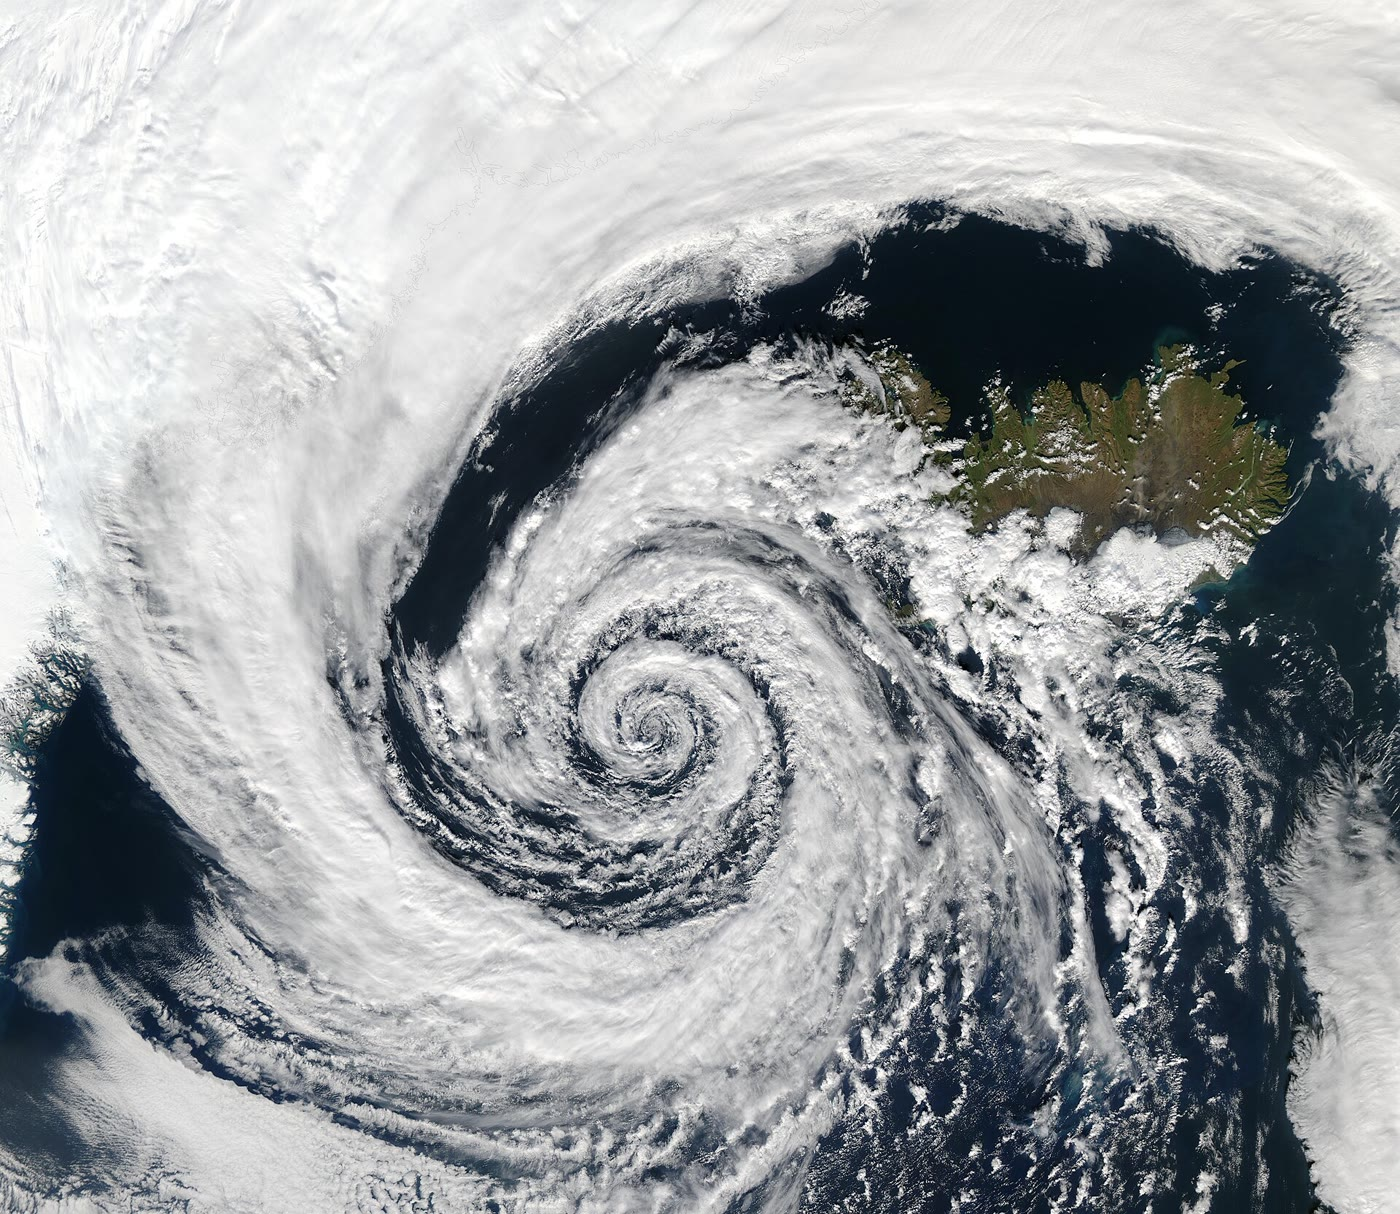
\includegraphics[width=\linewidth]{images/book5/b3-iceland-low.jpg}
\end{minipage}

\par\smallskip{\small बाएँ, तरंगदैर्घ्य के विरुद्ध ईडी वृद्धि दर, जनवरी के
\ang{45} N पर \omterm{def:b3:atmospheric-dynamics:eddy}{आंचलिक माध्य} अपरूपण के लिए (NCEP--NCAR पुनर्विश्लेषण~1,
1991--2020), क्षोभमंडल का माध्य स्तरीकरण और $H = \qty{11}{km}$:
\qty{3200}{km} से नीचे कोई वृद्धि नहीं, \qty{4700}{km} के निकट सबसे तेज़ वृद्धि। दाएँ, एक
परिपक्व चरण में अवदाब, आइसलैंड के दक्षिण-पश्चिम तट के पास, 4
सितंबर 2003; इसके बादल वामावर्त सर्पिल में निम्न-दाब के
चारों ओर लिपटे हैं (NASA/GSFC, MODIS Rapid Response Team, सार्वजनिक
डोमेन)।}\label{fig:b3:atmospheric-dynamics:eady}
\end{omfigure}
% ledger: data:b5-ncep-uwnd, nasa:grc-atmos, photo:b3-iceland-low

पुस्तक 4 (स्नातक वर्ष 2) का बहिरुष्णकटिबंधीय चक्रवात एक बढ़ती हुई \omterm{def:b3:gfd-foundations:baroclinic}{बैरोक्लिनिक} तरंग का सतही
पहलू है: इसका गर्म क्षेत्र गर्म हवा को ध्रुव की ओर और
ऊपर ले जाता है, इसके पीछे की ठंडी हवा भूमध्य रेखा की ओर और नीचे खिसकती है, और ऊपर का ट्रफ़
ऊँचाई के साथ पश्चिम की ओर झुकता है, जैसा कि \omterm{def:b3:atmospheric-dynamics:ape}{उपलब्ध स्थितिज
ऊर्जा} के मुक्त होने के लिए आवश्यक है।

\section{सामान्य परिसंचरण}\label{sec:b3:atmospheric-dynamics:general-circulation}

सामान्य परिसंचरण को अक्षांश वृत्तों के चारों ओर औसत लेकर वर्णित किया जाता है,
और औसत जो छोड़ देता है वह उतना ही महत्वपूर्ण है जितना वह जो रखता है।

\begin{definition}[आंचलिक माध्य और भँवर]\label{def:b3:atmospheric-dynamics:eddy}
किसी राशि $A$ का \emph{आंचलिक माध्य}\index{आंचलिक माध्य} स्थिर ऊँचाई या दाब पर
किसी अक्षांश वृत्त के चारों ओर उसका औसत है, $[A] =
(1/2\pi)\int_0^{2\pi} A\,\mathrm d\lambda$। विचलन $A^* = A - [A]$
उसका भँवर भाग है; वायुमंडल का \emph{भँवर}\index{भँवर (वायुमंडलीय)} वह
प्रवाह का अपने आंचलिक माध्य से हर विचलन है: गतिमान
तरंगें, स्थिर तरंगें, चक्रवात और प्रतिचक्रवात।
\end{definition}

किसी गुणनफल का \omterm{def:b3:atmospheric-dynamics:eddy}{आंचलिक माध्य} दो भागों में बँटता है: $[vT] = [v][T] + [v^*T^*]$। पहला
पद माध्य याम्योत्तर परिसंचरण द्वारा परिवहन है, यानी
पुस्तक 3 (स्नातक वर्ष 1) की कोष्ठिकाएँ; दूसरा पद भँवरों द्वारा परिवहन है। मध्य
अक्षांशों में माध्य याम्योत्तर पवन दुर्बल है और \omterm{def:b3:atmospheric-dynamics:eddy}{भँवर} पद
प्रबल होता है: ध्रुव की ओर बढ़ने वाली हवा उसी अक्षांश पर भूमध्य रेखा की ओर बढ़ने
वाली हवा से अधिक गर्म होती है, जैसा नीचे दिए चित्र में है, और $[v^*T^*] > 0$। \omterm{def:b3:atmospheric-dynamics:eddy}{भँवर} भी
पछुआ संवेग, $[u^*v^*]$, को उपोष्णकटिबंध से जेट धारा के
अक्षांशों तक ले जाते हैं, इसी कारण जेट धारा और भूतल पर पछुआ पवनें
घर्षण के विरुद्ध बनी रहती हैं। पुस्तक 3 (स्नातक वर्ष 1) की फ़ेरेल कोष्ठिका वह माध्य
याम्योत्तर परिसंचरण है जिसे यह \omterm{def:b3:atmospheric-dynamics:eddy}{भँवर} परिवहन प्रेरित करता है।

\begin{omfigure}
\begin{tikzpicture}[>=stealth, font=\small, declare function={s(\x)=0.9*sin(\x r); t(\x)=0.9*sin((\x+1.0) r);}]
\draw[thick, black, domain=0:12.566, samples=120] plot (\x, {s(\x)});
\draw[omThm, thick, densely dashed, domain=0:12.566, samples=120] plot (\x, {t(\x)-0.15});
\foreach \x in {0.3, 6.58} {\draw[->, omThm, very thick] (\x,-1.1) -- (\x,1.15)
  node[above, font=\scriptsize] {गर्म};}
\foreach \x in {3.45, 9.73} {\draw[->, omDef, very thick] (\x,1.1) -- (\x,-1.15)
  node[below, font=\scriptsize] {ठंडी};}
\node[font=\scriptsize, anchor=west] at (12.7,{s(12.566)}) {धारा-रेखा};
\node[font=\scriptsize, anchor=west, omThm] at (12.7,{t(12.566)-0.15}) {समतापी};
\draw[->] (-1.6,-1.1) -- (-0.6,-1.1) node[below, font=\scriptsize] {पूर्व};
\draw[->] (-1.6,-1.1) -- (-1.6,-0.1) node[above, font=\scriptsize] {उत्तर};
\node[font=\scriptsize] at (6.3,-1.95) {उत्तर में ठंडी हवा, दक्षिण में गर्म};
\end{tikzpicture}

\par\smallskip{\small एक बढ़ती हुई \omterm{def:b3:gfd-foundations:baroclinic}{बैरोक्लिनिक} तरंग का क्षैतिज दृश्य (योजनाबद्ध,
उत्तरी गोलार्ध, पछुआ प्रवाह)। समतापी रेखा (धराशायी) धारा-रेखा से
एक चौथाई तरंगदैर्घ्य या उससे कम पीछे रहती है, इसलिए उत्तर की ओर बढ़ने वाली हवा (लाल
तीर) उसी अक्षांश पर दक्षिण की ओर बढ़ने वाली हवा (नीले तीर) से अधिक गर्म है:
तरंग ध्रुव की ओर ऊष्मा ले जाती है, $[v^*T^*] >
0$।}\label{fig:b3:atmospheric-dynamics:heatflux}
\end{omfigure}

अयन वृत्त में \omterm{def:b3:atmospheric-dynamics:eddy}{भँवर} दुर्बल होते हैं और माध्य परिसंचरण ऊष्मा
ध्रुव की ओर ले जाता है, हैडली कोष्ठिका। पुस्तक 3 (स्नातक वर्ष 1) में पाया गया कि
भूमध्य रेखा से विराम अवस्था में निकलकर अपना कोणीय संवेग बनाए रखने वाली हवा सैकड़ों
मीटर प्रति सेकंड की गति से \ang{40} पर बहेगी, और यह प्रश्न खुला छोड़ा कि कोष्ठिका
\ang{30} के निकट क्यों समाप्त होती है। एक सरल मॉडल इसका उत्तर देता है।

\begin{definition}[वायुमंडलीय कोणीय संवेग; हेल्ड--हौ मॉडल]\label{def:b3:atmospheric-dynamics:held-hou}
\emph{वायुमंडलीय कोणीय संवेग}\index{वायुमंडलीय कोणीय संवेग} पृथ्वी की धुरी के चारों ओर प्रति इकाई द्रव्यमान
का मान $M = (\Omega a\cos\varphi +
u)\,a\cos\varphi$ है, पूर्व की ओर बहने वाली पवन $u$ के लिए, जो अक्षांश $\varphi$ पर है।
हैडली कोष्ठिका का \emph{हेल्ड--हौ मॉडल}\index{हेल्ड--हौ मॉडल} एक अक्षसममित, स्थायी
परिसंचरण है, जो एक शुष्क बूसिनेस्क वायुमंडल में होता है, जिसकी गहराई
$H$ है और जिसे शिथिलन द्वारा विकिरण-साम्य विभव
तापमान $\theta_E/\theta_0 = 1 + \Delta/3 - \Delta\sin^2\varphi$ की ओर तापित किया जाता है;
इसकी ऊपरी शाखा $M$ का संरक्षण करती है, निचली शाखा में नगण्य पवन होती है, और
प्रवाह \omterm{thm:b3:gfd-foundations:thermal-wind}{ऊष्मीय पवन} संतुलन में है।
\end{definition}

\begin{theorem}[हैडली कोष्ठिका का विस्तार]\label{thm:b3:atmospheric-dynamics:held-hou}
लघु-कोण सीमा में, हेल्ड--हौ कोष्ठिका उस अक्षांश तक पहुँचती है
\[
\varphi_H = \left(\frac{5\,gH\Delta}{3\,\Omega^2a^2}\right)^{1/2}
\]
प्रत्येक गोलार्ध में, और उसकी ऊपरी शाखा की पवन $u_M = \Omega
a\varphi^2$ है।
\end{theorem}

\begin{proof}
छोटे $\varphi$ पर, $\cos\varphi \approx 1$ और भूमध्य रेखा से विराम अवस्था में
निकलने वाली, $M = \Omega a^2$ वाली हवा के लिए $u_M = \Omega a(1 - \cos^2\varphi)/\cos\varphi
\approx \Omega a\varphi^2$। $f \approx 2\Omega\varphi$ और $y = a\varphi$ लेने पर,
भूतल पर कोई पवन नहीं, और \omterm{thm:b3:gfd-foundations:thermal-wind}{ऊष्मीय पवन} का बूसिनेस्क रूप
गहराई $H$ पर, $2\Omega\varphi\,u_M/H = -(g/a\theta_0)\,\partial\theta_M/
\partial\varphi$ है, जहाँ $\theta_M$ कोष्ठिका में $\theta$ का ऊर्ध्वाधर माध्य है।
तब $\partial(\theta_M/\theta_0)/\partial\varphi = -2\Omega^2a^2
\varphi^3/(gH)$ और $\theta_M/\theta_0 = A - K\varphi^4$, $K = \Omega^2a^2/
(2gH)$। कोष्ठिका के भीतर परिसंचरण ऊष्मा को केवल स्थानांतरित करता है, न उसे बनाता है न
नष्ट करता है, इसलिए कोष्ठिका का माध्य तापमान वही है जो विकिरण
साम्य का है: $\int_0^{\varphi_H}\theta_M\,\mathrm d\varphi = \int_0^{\varphi_H}
\theta_E\,\mathrm d\varphi$। उसकी सीमा पर तापमान सतत है:
$\theta_M(\varphi_H) = \theta_E(\varphi_H)$। $\theta_E/\theta_0 \approx
B - \Delta\varphi^2$, $B = 1 + \Delta/3$ लेने पर, पहली शर्त देती है $A - B =
K\varphi_H^4/5 - \Delta\varphi_H^2/3$, दूसरी शर्त $A - B = K\varphi_H^4 -
\Delta\varphi_H^2$। घटाने पर, $(4/5)K\varphi_H^4 = (2/3)\Delta
\varphi_H^2$, इसलिए $\varphi_H^2 = 5\Delta/(6K) = 5gH\Delta/(3\Omega^2a^2)$।
\end{proof}

कोष्ठिका वहाँ समाप्त होती है जहाँ कोणीय-संवेग संरक्षण द्वारा थोपा गया तापमान
विकिरण-साम्य से मिलता है; उससे आगे वायुमंडल को
विकिरण द्वारा बनाए गए तापमान से अधिक ठंडा होना पड़ता। मॉडल में दो प्राचल हैं, जो
प्रत्यक्ष रूप से नहीं देखे जाते। $H = \qty{15}{km}$ के लिए, और $\Delta$ का मान $1/6$ और
$1/3$ के बीच, उदाहरण के लिए चुने गए, $\varphi_H$ \ang{25} और \ang{35} के बीच है। देखे गए
\omterm{def:b3:atmospheric-dynamics:eddy}{आंचलिक माध्य} याम्योत्तर पवन से पढ़ी गई प्रेक्षित कोष्ठिकाएँ वार्षिक माध्य में
\ang{33.3} N और \ang{32.5} S पर समाप्त होती हैं, और शीतकालीन कोष्ठिकाएँ,
जो प्रबल हैं, \ang{30.8} N पर दिसंबर--फ़रवरी में और \ang{29.1} S पर
जून--अगस्त में समाप्त होती हैं। पैमाना ही मुख्य बात है: वह कोष्ठिका जो गहरे क्षोभमंडल
और प्रबल तापन अंतर के साथ चौड़ी होती है, और तेज़ी से घूमने वाले ग्रह पर
संकरी होती है। मॉडल की ऊपरी पवन, $u_M =
\qty{88}{m/s}$ है, $\Delta = 1/6$ के लिए उसकी सीमा पर, जो देखी गई
जेट धारा से दोगुनी है: अतिरिक्त को \omterm{def:b3:atmospheric-dynamics:eddy}{भँवर} दूर ले जाते हैं।
% ledger: geod5:grs80-defining, earth:Rmean, data:b5-ncep-vwnd (values in figdata/bachelor-3/held_hou.py)

\begin{omfigure}
\begin{tikzpicture}
\begin{groupplot}[group style={group size=2 by 1, horizontal sep=1.7cm},
  width=0.48\linewidth, height=0.44\linewidth, tick label style={font=\scriptsize},
  label style={font=\small}, legend style={font=\scriptsize, draw=none, fill=none}]
\nextgroupplot[xlabel={अक्षांश (\unit{\degree})}, ylabel={$100\,(\theta/\theta_0 - 1)$},
  xmin=0, xmax=60, ymin=-30, ymax=15, legend pos=south west, legend cell align=left,
  title={\small $\Delta = 1/3$, $H = \qty{15}{km}$}]
% computed in figdata/bachelor-3/held_hou.py
\addplot[omDef, thick] table[x=phi, y=thE] {figdata/out/bachelor-3-held_hou-theta-3.dat};
\addplot[omThm, thick, unbounded coords=jump] table[x=phi, y=thM] {figdata/out/bachelor-3-held_hou-theta-3.dat};
\addplot[black!50, densely dashed, forget plot] coordinates {(35.26,-30) (35.26,15)};
\node[font=\scriptsize, anchor=south west] at (axis cs:35.6,7) {$\varphi_H$};
\legend{$\theta_E$, $\theta_M$}
\nextgroupplot[xlabel={अक्षांश (\unit{\degree})}, ylabel={$\psi$ \qty{500}{hPa} पर ($10^{10}$\,\unit{kg/s})},
  xmin=-60, xmax=60, ymin=-25, ymax=25, xtick={-60,-30,0,30,60}, legend pos=south west,
  legend cell align=left]
\addplot[black!50, thin, domain=-60:60, samples=2, forget plot] {0};
\addplot[black, thick] table[x=lat, y=ann] {figdata/out/bachelor-3-held_hou-psi.dat};
\addplot[omDef, thick] table[x=lat, y=djf] {figdata/out/bachelor-3-held_hou-psi.dat};
\addplot[omThm, thick] table[x=lat, y=jja] {figdata/out/bachelor-3-held_hou-psi.dat};
\legend{वर्ष, दिसं--फ़र, जून--अग}
\end{groupplot}
\end{tikzpicture}

\par\smallskip{\small बाएँ, हैडली--हौ रचना: कोष्ठिका का कोणीय-संवेग-संरक्षी तापमान (लाल)
विकिरण साम्य (नीला) से $\varphi_H = \ang{35}$ पर मिलता है, कोष्ठिका के भीतर के
वक्रों के बीच समान क्षेत्रफल रखते हुए। दाएँ, \qty{500}{hPa} पर माध्य याम्योत्तर
द्रव्यमान धारा-फलन, \omterm{def:b3:atmospheric-dynamics:eddy}{आंचलिक माध्य} याम्योत्तर पवन से (NCEP--NCAR
पुनर्विश्लेषण~1, 1991--2020; धनात्मक जहाँ \qty{500}{hPa} से ऊपर की वायु उत्तर की ओर बढ़ती है): प्रबल
शीत-गोलार्ध कोष्ठिका भूमध्य रेखा को पार करती है,
और कोष्ठिकाएँ
\ang{30} के आसपास
समाप्त होती हैं।}\label{fig:b3:atmospheric-dynamics:held-hou}
\end{omfigure}
% ledger: data:b5-ncep-vwnd

\begin{history}[दीर्घ तरंगों से पहले संगणित पूर्वानुमान तक]
वर्ष 1939 में C.-G.~रॉस्बी और उनके सहयोगियों ने \emph{Journal of Marine Research}
में मौसम की कई प्रतीत होने वाली स्वतंत्र घटनाओं को एक ही दृष्टिकोण से समझाने का प्रयास किया।
मौसम के उन प्रारूपों से प्रेरित होकर, जो प्रचलित पछुआ प्रवाह के विरुद्ध
उजानी की ओर बढ़ते हैं, रॉस्बी ने एक रैखिक सिद्धांत लिखा, जिसमें
बड़े पैमाने के विक्षोभ पश्चिम की ओर बढ़ने की प्रवृत्ति रखते हैं, और
छोटे विक्षोभ पवन के सापेक्ष पूर्व की ओर; यही इस अध्याय की तरंगें और
$\beta$-समतल हैं। ग्यारह वर्ष बाद J.~G.~चार्नी,
R.~फ़्योरटॉफ़्ट और J.~फ़ॉन~न्यूमैन ने \omterm{thm:b3:atmospheric-dynamics:bve}{बैरोट्रॉपिक भ्रमिलता समीकरण} का
ENIAC इलेक्ट्रॉनिक कंप्यूटर पर संख्यात्मक समाकलन किया: 24~घंटे के चार पूर्वानुमान
\qty{500}{mb} स्तर पर, \qty{736}{km} के ग्रिड पर, देशांतर के 8 अंश,
\ang{45} पर। प्रत्येक पूर्वानुमान की गणना में लगभग 24~घंटे लगे:
जैसा उन्होंने लिखा, वे मौसम की गति से बस आगे रह पाए।
\end{history}
% ledger: rossby39:paper, jmr20:commentary, charney50:eniac

\section{अभ्यास}

\begin{exercise}[$\star$]\label{exo:b3:atmospheric-dynamics:1}
(क)~ठोस घूर्णन में एक \omterm{def:b3:atmospheric-dynamics:eddy}{भँवर} की \omterm{def:b3:atmospheric-dynamics:vorticity-kinds}{आपेक्षिक भ्रमिलता} परिकलित कीजिए, जो
एक दिन में एक बार घूमता है। (ख)~\ang{30} और \ang{60} N पर \omterm{def:b3:atmospheric-dynamics:vorticity-kinds}{ग्रहीय भ्रमिलता}
($\Omega = \qty{7.292e-5}{rad/s}$) परिकलित कीजिए और तुलना कीजिए।
\end{exercise}

\begin{exercise}[$\star$]\label{exo:b3:atmospheric-dynamics:2}
\ang{30} N पर शून्य \omterm{def:b3:atmospheric-dynamics:vorticity-kinds}{आपेक्षिक भ्रमिलता} वाला एक वायु-कण
बिना अपसरण वाले प्रवाह में \ang{40} N तक जाता है। वहाँ उसकी \omterm{def:b3:atmospheric-dynamics:vorticity-kinds}{आपेक्षिक भ्रमिलता} परिकलित कीजिए। क्या वह
चक्रवाती है या प्रतिचक्रवाती?
\end{exercise}

\begin{exercise}[$\star$]\label{exo:b3:atmospheric-dynamics:3}
\ang{45} N पर, बिना माध्य पवन के, एक रॉस्बी तरंग की
तरंगदैर्घ्य \qty{5000}{km} और $l = 0$ है, कला-चाल परिकलित कीजिए। वह किस दिशा में चलती है?
\end{exercise}

\begin{exercise}[$\star$]\label{exo:b3:atmospheric-dynamics:4}
\ang{60} N पर \qty{10}{m/s} की पछुआ में $\beta$, स्थिर
तरंगदैर्घ्य और अक्षांश वृत्त के चारों ओर स्थिर तरंगों की संख्या
($a = \qty{6371}{km}$) परिकलित कीजिए।
\end{exercise}

\begin{exercise}[$\star\star$]\label{exo:b3:atmospheric-dynamics:5}
\qty{10}{km} गहरा वायु का स्तंभ, \ang{45} N पर बिना \omterm{def:b3:atmospheric-dynamics:vorticity-kinds}{आपेक्षिक भ्रमिलता} के,
एक पर्वत-श्रेणी को पार करता है, जो उसे \qty{8}{km} तक संपीड़ित कर देती है; फिर
एक द्रोणी, जहाँ वह \qty{12}{km} गहरा है। मानिए कि वह \ang{45} N के समीप रहता है, तो
पर्वत-श्रेणी और द्रोणी के ऊपर उसकी \omterm{def:b3:atmospheric-dynamics:vorticity-kinds}{आपेक्षिक भ्रमिलता} परिकलित कीजिए। अवदाब
कहाँ बनने की प्रवृत्ति रखेंगे?
\end{exercise}

\begin{exercise}[$\star\star$]\label{exo:b3:atmospheric-dynamics:6}
\ang{45} N वृत्त के चारों ओर पाँच शिखरों वाली तरंग के लिए ($l = 0$),
\qty{15}{m/s} की पछुआ में, कला-चाल और समूह वेग परिकलित कीजिए।
तरंग की ऊर्जा को \qty{5000}{km} पूर्व की ओर जाने में कितना समय लगता है, और
प्रारूप को कितना समय लगता है?
\end{exercise}

\begin{exercise}[$\star\star$]\label{exo:b3:atmospheric-dynamics:7}
\ang{45} N पर \qty{15}{m/s} की पछुआ में एक तरंग अक्षांशों के बीच इस प्रकार सीमित है
कि $l = \pi/(\qty{6000}{km})$ हो। (क)~उसकी स्थिर आंचलिक तरंग-संख्या और तरंगदैर्घ्य परिकलित कीजिए।
(ख)~दिखाइए कि
$l = \pi/(\qty{3000}{km})$ के लिए कोई स्थिर तरंग नहीं होती।
\end{exercise}

\begin{exercise}[$\star\star$]\label{exo:b3:atmospheric-dynamics:8}
\ang{45} N पर एक \omterm{def:b3:atmospheric-dynamics:eady}{ईडी मॉडल} में $\Lambda = \qty{2e-3}{s^{-1}}$, $N =
\qty{0.012}{s^{-1}}$ और $H = \qty{10}{km}$ है। सबसे तेज़ी से बढ़ने वाले विक्षोभ का $L_d$,
वृद्धि दर और $e$-गुणन काल, तथा
उसकी तरंगदैर्घ्य परिकलित कीजिए।
\end{exercise}

\begin{exercise}[$\star\star$]\label{exo:b3:atmospheric-dynamics:9}
अक्षांश वृत्त के साथ \omterm{def:b3:atmospheric-dynamics:eddy}{भँवर} याम्योत्तर पवन $v^* = V\cos kx$ है और
\omterm{def:b3:atmospheric-dynamics:eddy}{भँवर} तापमान $T^* = T_0\cos(kx - \delta)$ है, जहाँ
$V = \qty{10}{m/s}$ और $T_0 = \qty{5}{K}$ है। $[v^*T^*]$ को $\delta = 0$, \ang{60} और
\ang{90} के लिए परिकलित कीजिए, और संगत ऊष्मा फ़्लक्स $\rho c_p[v^*T^*]$, वायु के
प्रति \unit{kg/m^3} ($c_p = \qty{1004}{J.kg^{-1}.K^{-1}}$) के लिए परिकलित कीजिए। कौन-सी
व्यवस्था कोई ऊष्मा परिवहन नहीं करती?
\end{exercise}

\begin{exercise}[$\star\star\star$]\label{exo:b3:atmospheric-dynamics:10}
\omterm{thm:b3:atmospheric-dynamics:bve}{बैरोट्रॉपिक भ्रमिलता समीकरण} से आरंभ करके एक समान पछुआ पवन में रॉस्बी तरंगों का
परिक्षेपण संबंध व्युत्पन्न कीजिए, और दिखाइए कि वायु के सापेक्ष हर रॉस्बी तरंग
पश्चिम की ओर चलती है।
\end{exercise}

\begin{exercise}[$\star\star\star$]\label{exo:b3:atmospheric-dynamics:11}
\omterm{def:b3:atmospheric-dynamics:held-hou}{हेल्ड--हौ मॉडल} में $H = \qty{12}{km}$ और $\Delta = 1/4$ लीजिए।
$\varphi_H$, किनारे पर लघु-कोण पवन $u_M$ और वहाँ की सटीक कोणीय-संवेग पवन
परिकलित कीजिए, और उसकी तुलना जनवरी के \omterm{def:b3:atmospheric-dynamics:eddy}{आंचलिक माध्य} की
\qty{44}{m/s} वाले उपोष्णकटिबंधीय जेट से कीजिए।
\end{exercise}

\begin{exercise}[$\star\star\star$]\label{exo:b3:atmospheric-dynamics:12}
वायु की दो परतों का विभव तापमान \qty{300}{K} पर \qty{10}{K} भिन्न है;
उनका अंतरापृष्ठ ढलान $s$ के साथ ध्रुव की ओर ऊपर उठता है, और यह \qty{4000}{km}
चौड़ी पट्टी के पार है, तथा $\rho = \qty{0.7}{kg/m^3}$। (क)~दिखाइए कि अंतरापृष्ठ के
समतल होने देने पर $\rho g' s^2L^2/24$ प्रति इकाई
क्षेत्रफल मुक्त होता है, जहाँ $g' = g\,\Delta\theta/\theta$। (ख)~$s = 10^{-3}$ और $2\times10^{-3}$ के लिए
इसका परिकलन कीजिए और उसकी तुलना उसी वायु की \qty{10}{km} मोटाई से होकर
बहती \qty{15}{m/s} की पवन की गतिज ऊर्जा से कीजिए।
\end{exercise}
% ledger: geod5:grs80-defining, earth:Rmean, data:b5-ncep-uwnd

\section{समस्या: वह तरंग जो स्थिर रही}

\begin{problem}[{सप्ताहांत समस्या --- भ्रमिलता, रॉस्बी तरंगें और
\ang{45} N पर \omterm{def:b3:gfd-foundations:baroclinic}{बैरोक्लिनिक} तरंग की वृद्धि}]
\label{pb:b3:atmospheric-dynamics:1}
\qty{15}{m/s} का एक पछुआ प्रवाह एक काल्पनिक महाद्वीप के मध्य अक्षांशों को पार करता है,
\ang{45} N के साथ-साथ। मान लीजिए $\Omega =
\qty{7.292115e-5}{rad/s}$, $a = \qty{6371}{km}$ और $g = \qty{9.81}{m/s^2}$।
प्रवाह के सभी मान काल्पनिक हैं।

\medskip\noindent\textbf{भाग I --- विस्थापित वायु-पिंड।}
\begin{enumerate}
\item \ang{45} N पर \omterm{def:b3:atmospheric-dynamics:vorticity-kinds}{आपेक्षिक भ्रमिलता} रहित एक वायु-पिंड को
  \ang{50} N तक धकेला जाता है। दोनों अक्षांशों पर $f$ और
  यदि प्रवाह में अपसरण न हो, तो \ang{50} N पर उसकी \omterm{def:b3:atmospheric-dynamics:vorticity-kinds}{आपेक्षिक भ्रमिलता} परिकलित कीजिए।
\item \qty{15}{m/s} की गति से चलते हुए यह किस वक्रता-त्रिज्या पर मुड़ता है
  (मान लीजिए $\zeta = -V/R$, और यह पूरी तरह वक्रता से है)? किस ओर मुड़ता है?
\item यदि इस मार्ग में इसका स्तंभ भी \qty{10.0}{km} से घटकर \qty{9.5}{km} रह जाता है,
  तो \ang{50} N पर इसकी \omterm{def:b3:atmospheric-dynamics:vorticity-kinds}{आपेक्षिक भ्रमिलता} क्या होगी?
\item इसके बजाय \ang{40} N तक धकेले जाने पर, बिना अपसरण के, यह
  कितनी \omterm{def:b3:atmospheric-dynamics:vorticity-kinds}{आपेक्षिक भ्रमिलता} प्राप्त करता है? समझाइए कि अपने अक्षांश से विस्थापित वायु-पिंड
  उसी के चारों ओर क्यों दोलन करता है।
\end{enumerate}

\medskip\noindent\textbf{भाग II --- गतिमान तरंगें।}
\begin{enumerate}[resume]
\item \ang{45} N पर $\beta$ और अक्षांश वृत्त की लंबाई परिकलित कीजिए।
\item वृत्त के चारों ओर $n = 3$ से 8 तरंगों के लिए ($l = 0$),
  \qty{15}{m/s} की पछुआ में तरंगदैर्घ्य, कला-वेग
  और समूह वेग परिकलित कीजिए।
\item कौन-सी तरंगें पश्चिम की ओर और कौन-सी पूर्व की ओर चलती हैं? तरंग
  $n = 5$ को \qty{1000}{km} चलने में कितने दिन लगते हैं?
\item महाद्वीप के पश्चिम में एक कटक प्रबल होता है। कहाँ, और
  कितने समय बाद, $n = 6$ तरंग का प्रभाव \qty{5000}{km}
  नीचे की ओर पहुँचेगा?
\end{enumerate}

\medskip\noindent\textbf{भाग III --- वह तरंग जो स्थिर रही।}
\begin{enumerate}[resume]
\item स्थिर तरंगदैर्घ्य और स्थिर तरंग-संख्या
  \ang{45} N पर परिकलित कीजिए।
\item 10 और
  \qty{20}{m/s} की पछुआ पवनों के लिए स्थिर तरंग-संख्या परिकलित कीजिए। शीतकाल में जब
  पछुआ पवनें प्रबल होती हैं, तो स्थिर तरंगों का क्या होता है?
\item \ang{35} N और \ang{55} N पर स्थिर तरंग-संख्या
  \qty{15}{m/s} की पछुआ में परिकलित कीजिए।
\item महाद्वीप के पश्चिमी पर्वत \qty{10}{km} गहरे क्षोभमंडल में
  \qty{2}{km} ऊँचे उठते हैं। अक्षांश बदले बिना उन्हें पार करने वाले स्तंभ की
  \omterm{def:b3:atmospheric-dynamics:vorticity-kinds}{आपेक्षिक भ्रमिलता} परिकलित कीजिए। पर्वत स्थिर तरंगों को क्यों
  प्रेरित करते हैं?
\item पर्वतों द्वारा प्रेरित तरंग-प्रारूप केवल तभी स्थिर क्यों रहता है,
  जब उसकी तरंगदैर्घ्य $\lambda_s$ के निकट हो?
\end{enumerate}

\medskip\noindent\textbf{भाग IV --- एक तूफ़ान बढ़ता है।}
\begin{enumerate}[resume]
\item धरातल से \qty{10}{km} तक पछुआ पवन में
  \qty{25}{m/s} की वृद्धि होती है। अपरूपण $\Lambda$ तथा ध्रुव की ओर की तापमान
  प्रवणता परिकलित कीजिए, जो \qty{250}{K} के माध्य तापमान पर \omterm{thm:b3:gfd-foundations:thermal-wind}{ऊष्मीय पवन} के
  अनुसार इस अपरूपण से निहित होती है।
\item $N = \qty{0.011}{s^{-1}}$ लेकर रिचर्डसन संख्या
  $N^2/\Lambda^2$ परिकलित कीजिए। क्या प्रवाह लघु-पैमाने की अपरूपण प्रक्षुब्धता के प्रति अस्थिर है?
\item रॉस्बी त्रिज्या $L_d$ परिकलित कीजिए, जहाँ $H = \qty{10}{km}$ है।
\item सबसे तेज़ बढ़ने वाले ईडी विक्षोभ की तरंगदैर्घ्य
  और अक्षांश वृत्त के चारों ओर ऐसी तरंगों की संख्या परिकलित कीजिए।
\item बढ़ने वाली सबसे छोटी तरंगदैर्घ्य परिकलित कीजिए।
\item वृद्धि दर $\sigma_{\max}$ परिकलित कीजिए।
\item तीन दिन में विक्षोभ किस गुणक से बढ़ता है?
\item बढ़ते तूफ़ान की तरंगदैर्घ्य की तुलना भाग~III की स्थिर
  तरंगदैर्घ्य से कीजिए: कौन-सी लंबी है, और इससे स्थिर तरंगों के सापेक्ष तूफ़ानों की
  गति के बारे में क्या निष्कर्ष निकलता है?
\item बढ़ती तरंग का गर्त ऊँचाई के साथ किस ओर झुकता है,
  और ऐसा क्यों होना अनिवार्य है?
\item सबसे तेज़ बढ़ने वाले ईडी विक्षोभ का $e$-गुणन काल दीजिए।
\end{enumerate}
\end{problem}
% ledger: geod5:grs80-defining, earth:Rmean
